\vspace{-0.3em}
\begin{block}{Stochastic Block Model (Counting-Generator)} %: Random Community Assignment}

\textbf{Model:} Each $v$ is assigned to a \emph{random} community (color) from $C_1, \ldots, C_r$.

\quad$\Rightarrow$ If $u\in C_i, v\in C_j$, then $\mathbb {P}[{(u, v)\in E}] = p_{ij}$.
($|C_i|$'s are given as input)

\vspace{15pt}

\colorbox{CornflowerBlue}{\textbf{Idea \#1}} use \#nodes of each color in \emph{any} contiguous range to generate SBM

\vspace{-0.5in}
\begin{figure}[h]
    \centering
    \fcolorbox{CornflowerBlue}{white}{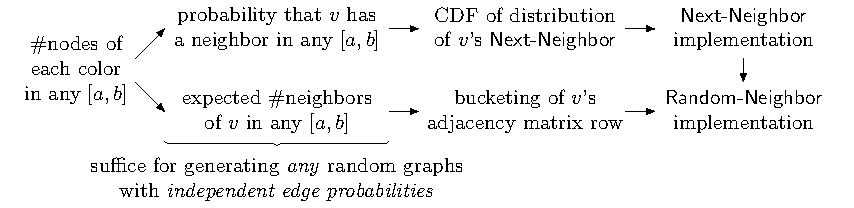
\includegraphics[width=\textwidth]{svg/fig2.pdf}}
\end{figure}

\colorbox{CornflowerBlue}{\textbf{Idea \#2}} implement a \textbf{Counting-Generator} to answer counting queries

\quad$\Rightarrow$ BBST, split on-the-fly with \emph{Multivariate Hypergeometric Distribution}



\iffalse{

%\begin{itemize}
    %\item Each vertex is assigned to some community $C_i\subseteq V$ for $i\in [r]$
%Communities $\{C_i\}_{i\in [r]}$ partition $V$: If $u\in C_i, v\in C_j$, then $\mathbb P_{(u, v)\in E} = p_{ij}$.
    %where $\left\{ p_{ij}\right\}_{i,j\in [r]}\in [0,1]^{r\times r}$
%\end{itemize}
\begin{itemize}
\item [] \textbf{Given sizes of each comunity $C_i$ and a range of length $\ell$}
    \item Count number of occurrences of each community in any contiguous range%: $|[a,b]\cap C_j|$
    \item Sample from \emph{Multivariate Hypergeometric Distribution}%: $O(r\, poly(\log n))$ resources
\[
\Pr[\mathbf{S}^\mathbf{C}_\ell = \langle s_1, \ldots, s_r \rangle]
= \frac{\binom{C_1}{s_1}\cdot\binom{C_2}{s_2}\cdots\binom{C_r}{s_r}}{\binom{B}{\ell}}
\hspace{2ex}\textrm{ where } \scriptstyle{
    \ell = \mathlarger{\sum}\limits^{r}_{i=1} s_i \textrm{ and } B = \mathlarger{\sum}\limits^{r}_{i=1} C_i
}
\]
\end{itemize}

\fi


\vspace{0.5em}
\begin{figure}[h!]\centering
    \def\svgwidth{0.93\columnwidth}
    \import{svg/}{counting.pdf_tex}
\end{figure}


\end{block}
